\documentclass[12pt]{article}
\extrafloats{100}
\usepackage{a4wide}
\usepackage{booktabs}
\usepackage{multicol, multirow}
\usepackage[cp1251]{inputenc}
\usepackage[russian]{babel}
\usepackage{amsmath, amsfonts, amssymb, amsthm, amscd}
\usepackage{graphicx, epsfig, subfig, epstopdf}
\usepackage{longtable}
\graphicspath{ {../fig/} {../} {fig/} {decompose/}}
\begin{document}


{\tiny 
 \begin{tabular}{lrrrllrr}
\toprule
{} &  N. obs. &     Min &     Max &                        T. min &                         T.max &        T. delta &  Nans \\
\midrule
11473 &     5088 &  143.10 &  146.43 & 1970-01-01 00:00:01.392136578 & 1970-01-01 00:00:01.399615365 & 00:00:00.000000 &     0 \\
11474 &     5088 &   37.00 &   38.00 & 1970-01-01 00:00:01.392136578 & 1970-01-01 00:00:01.399615365 & 00:00:00.000000 &     0 \\
11505 &     5088 &  112.08 &  120.87 & 1970-01-01 00:00:01.392136578 & 1970-01-01 00:00:01.399615365 & 00:00:00.000000 &     0 \\
11506 &     5088 &   29.00 &   31.00 & 1970-01-01 00:00:01.392136578 & 1970-01-01 00:00:01.399615365 & 00:00:00.000000 &     0 \\
11508 &     5149 &   71.00 &   80.00 & 1970-01-01 00:00:01.392136578 & 1970-01-01 00:00:01.399615365 & 00:00:00.000000 &     0 \\
11507 &     5149 &   35.64 &   39.88 & 1970-01-01 00:00:01.392136578 & 1970-01-01 00:00:01.399615365 & 00:00:00.000000 &     0 \\
\bottomrule
\end{tabular}

 }
 \bigskip 
11473: Estimated period 100.0 with std 0.0 \\ 

\begin{figure}
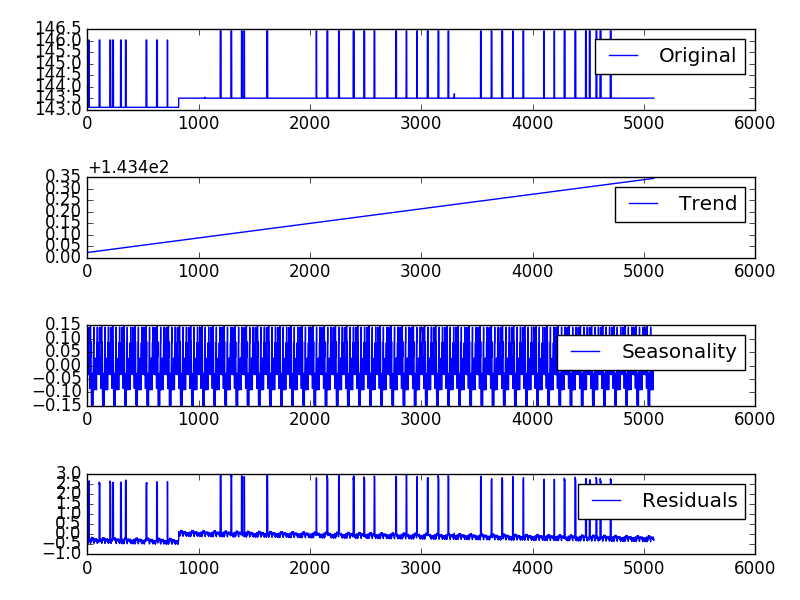
\includegraphics[width=0.9\textwidth]{11473/decomposition.png}
\caption{Decomposition of time series into trend and seasonal component).} \label{fg:decomp}
\end{figure}

\begin{figure}
\subfloat{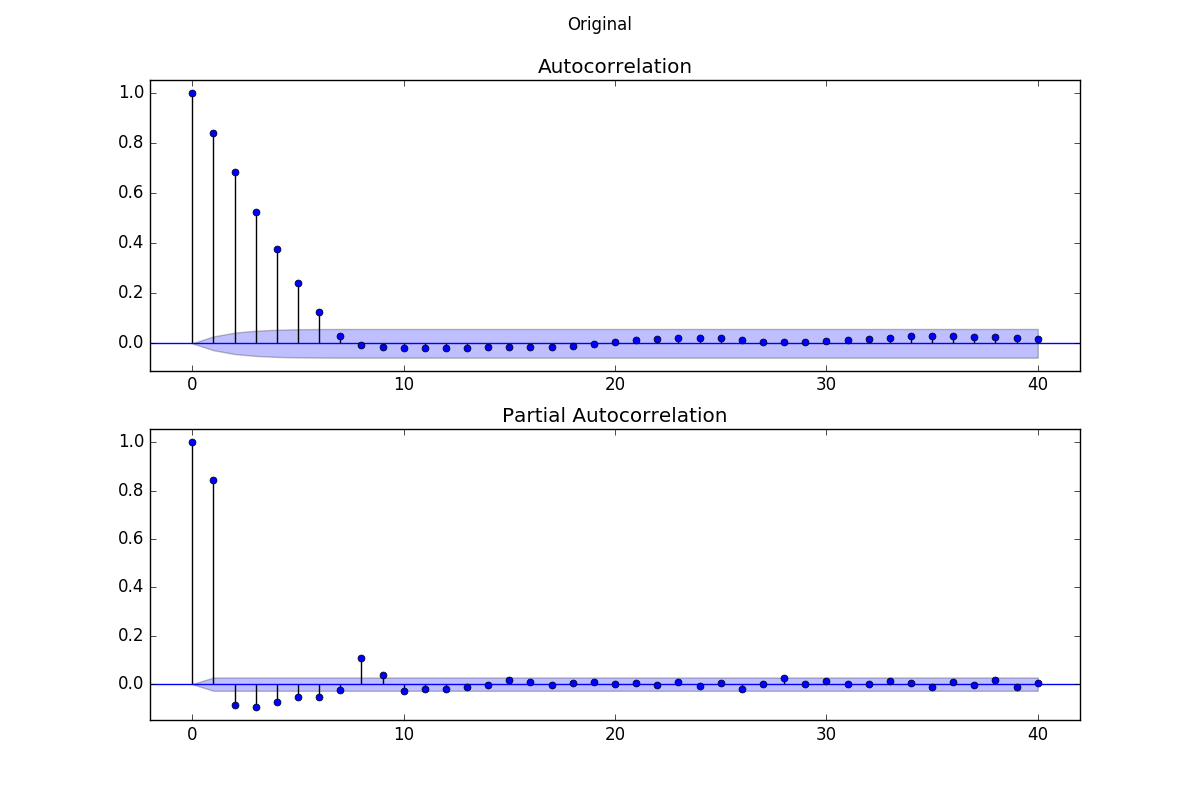
\includegraphics[width=0.5\textwidth]{11473/acf_Original.png}}
\subfloat{\includegraphics[width=0.5\textwidth]{11473/acf_Trend.png}}\\ 
\subfloat{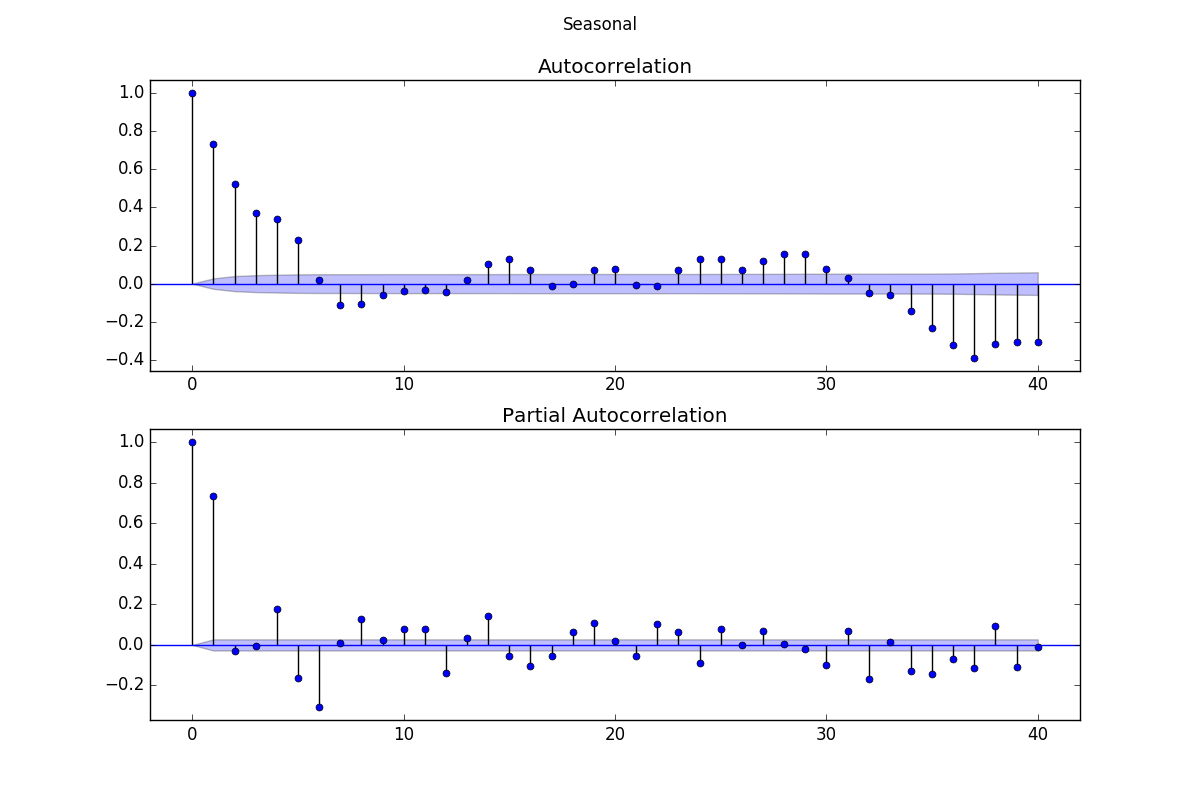
\includegraphics[width=0.5\textwidth]{11473/acf_Seasonal.png}}
\subfloat{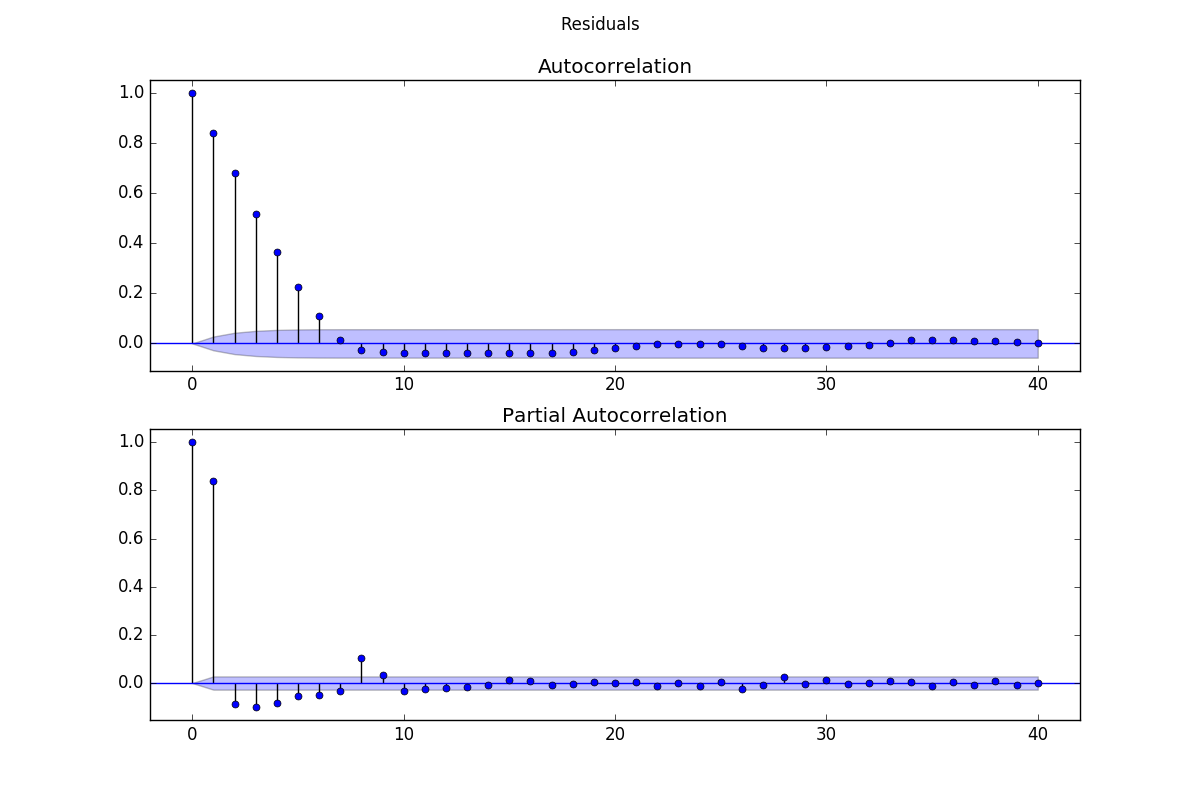
\includegraphics[width=0.5\textwidth]{11473/acf_Residuals.png}}
\caption{ACF and PACF for componets of the time series.} \label{fg:acf}
\end{figure}
11474: Estimated period 100.0 with std 0.0 \\ 

\begin{figure}
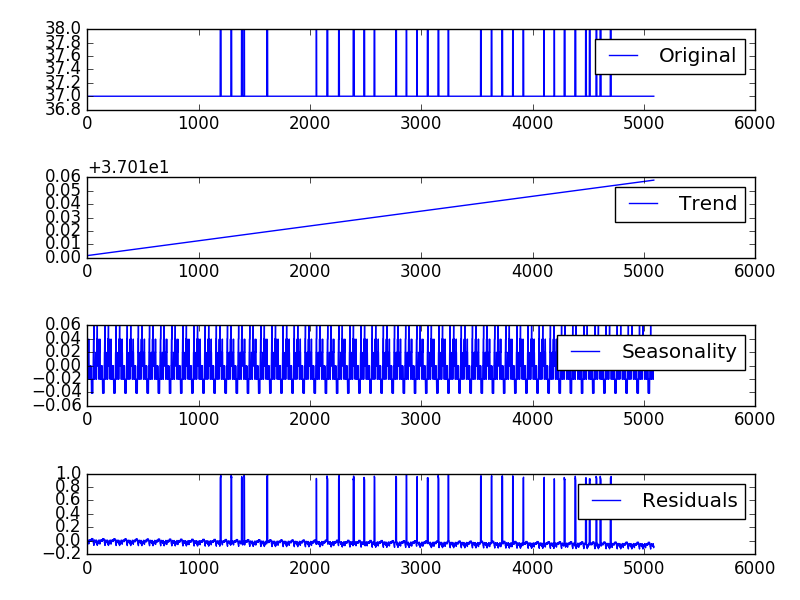
\includegraphics[width=0.9\textwidth]{11474/decomposition.png}
\caption{Decomposition of time series into trend and seasonal component).} \label{fg:decomp}
\end{figure}

\begin{figure}
\subfloat{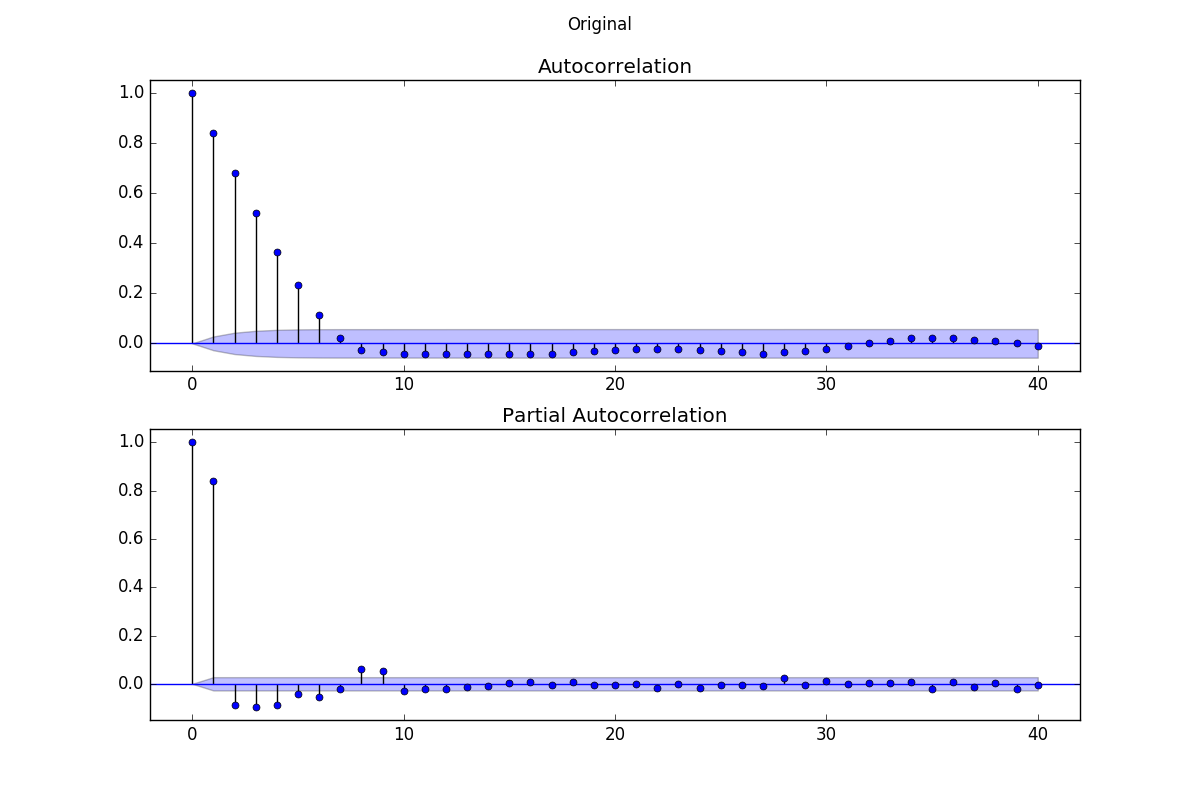
\includegraphics[width=0.5\textwidth]{11474/acf_Original.png}}
\subfloat{\includegraphics[width=0.5\textwidth]{11474/acf_Trend.png}}\\ 
\subfloat{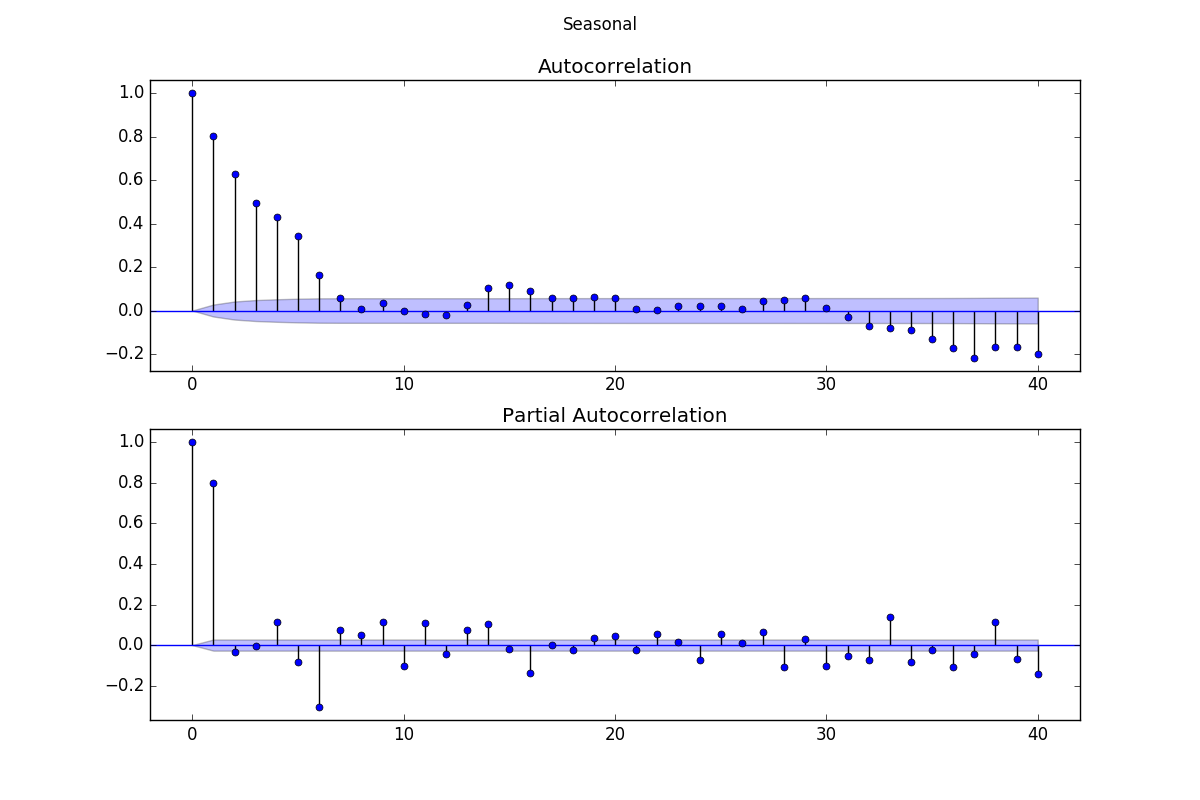
\includegraphics[width=0.5\textwidth]{11474/acf_Seasonal.png}}
\subfloat{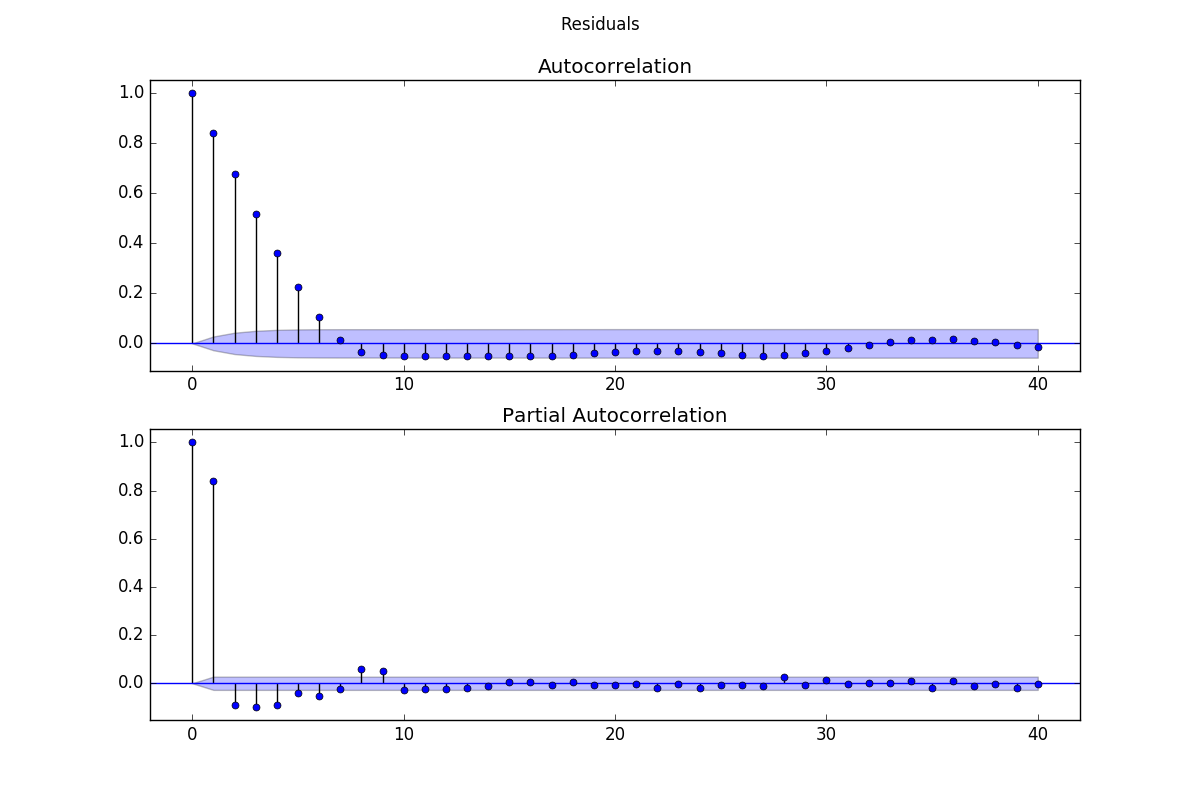
\includegraphics[width=0.5\textwidth]{11474/acf_Residuals.png}}
\caption{ACF and PACF for componets of the time series.} \label{fg:acf}
\end{figure}
11505: Estimated period 100.0 with std 0.0 \\ 

\begin{figure}
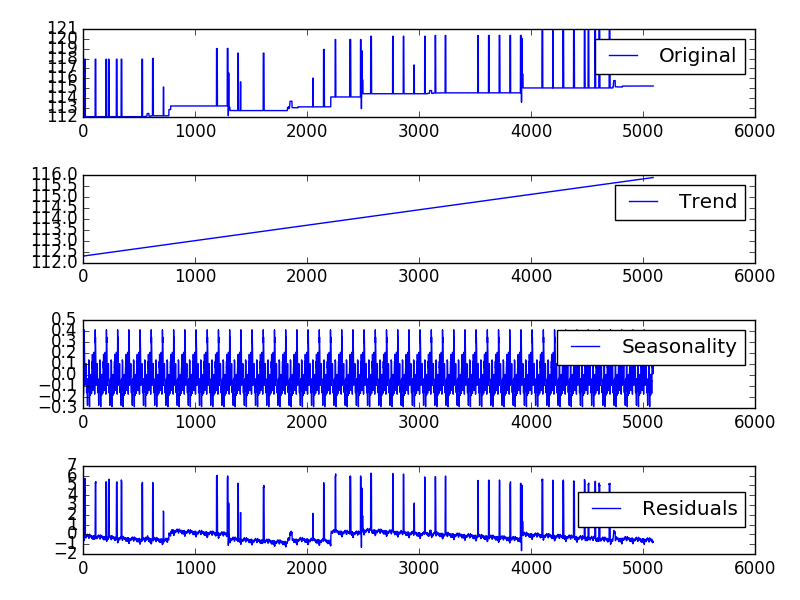
\includegraphics[width=0.9\textwidth]{11505/decomposition.png}
\caption{Decomposition of time series into trend and seasonal component).} \label{fg:decomp}
\end{figure}

\begin{figure}
\subfloat{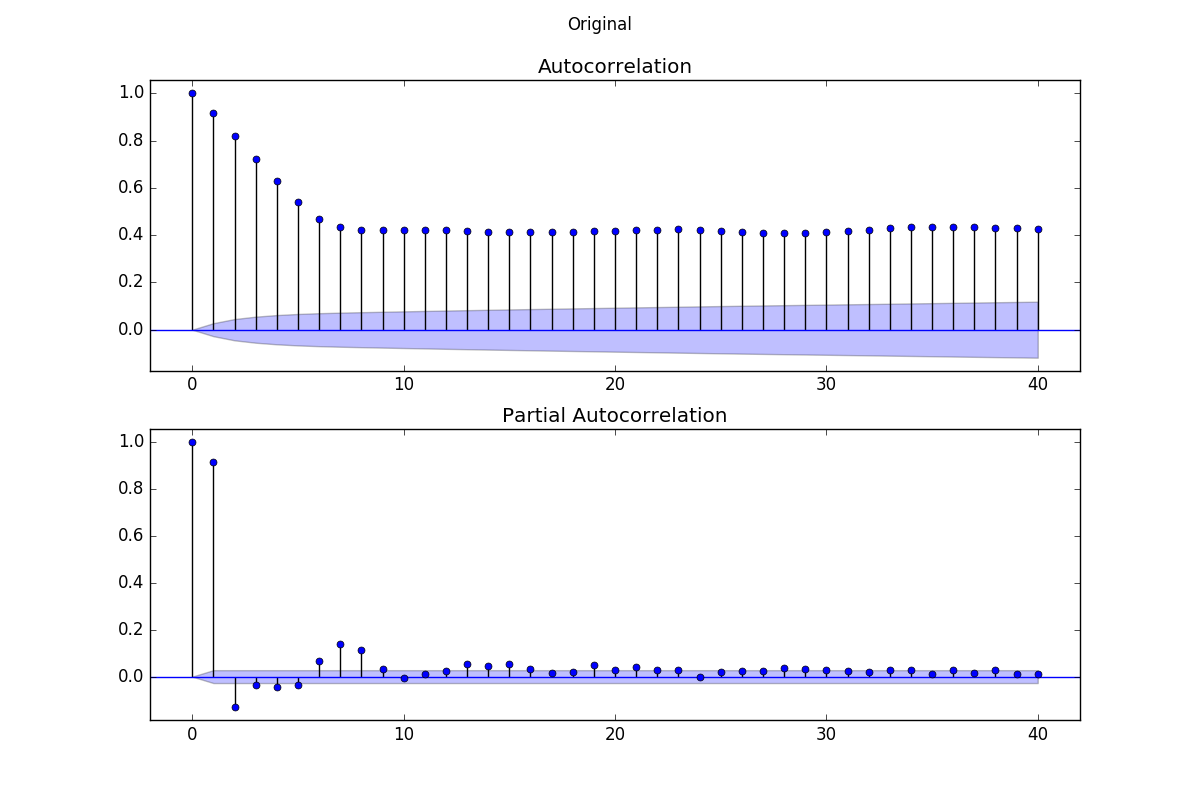
\includegraphics[width=0.5\textwidth]{11505/acf_Original.png}}
\subfloat{\includegraphics[width=0.5\textwidth]{11505/acf_Trend.png}}\\ 
\subfloat{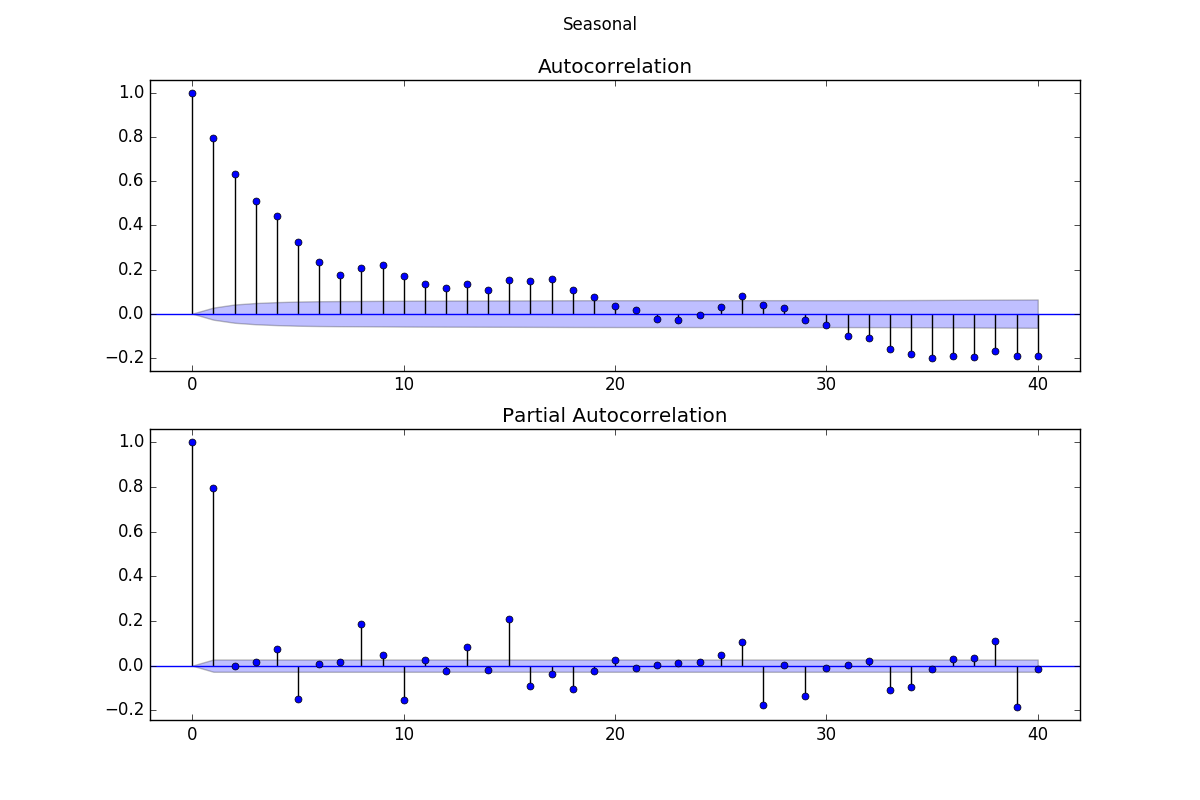
\includegraphics[width=0.5\textwidth]{11505/acf_Seasonal.png}}
\subfloat{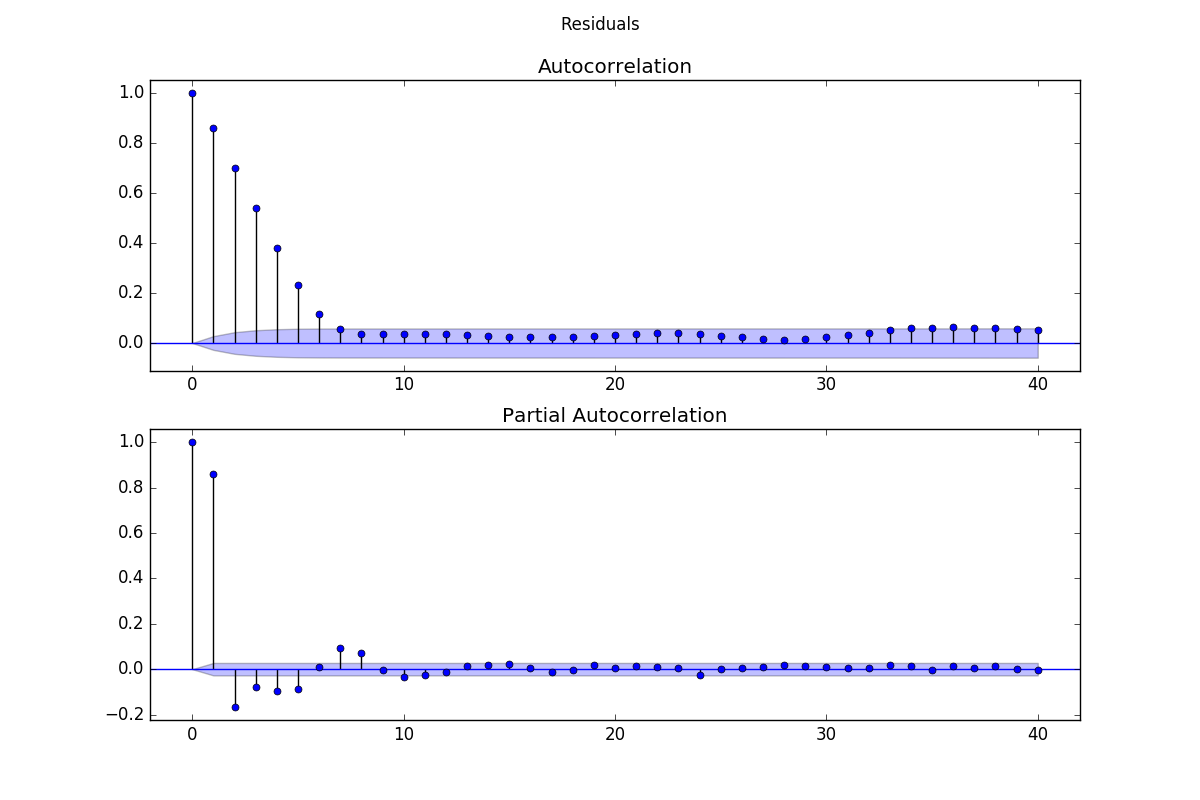
\includegraphics[width=0.5\textwidth]{11505/acf_Residuals.png}}
\caption{ACF and PACF for componets of the time series.} \label{fg:acf}
\end{figure}
11506: Estimated period 100.0 with std 0.0 \\ 

\begin{figure}
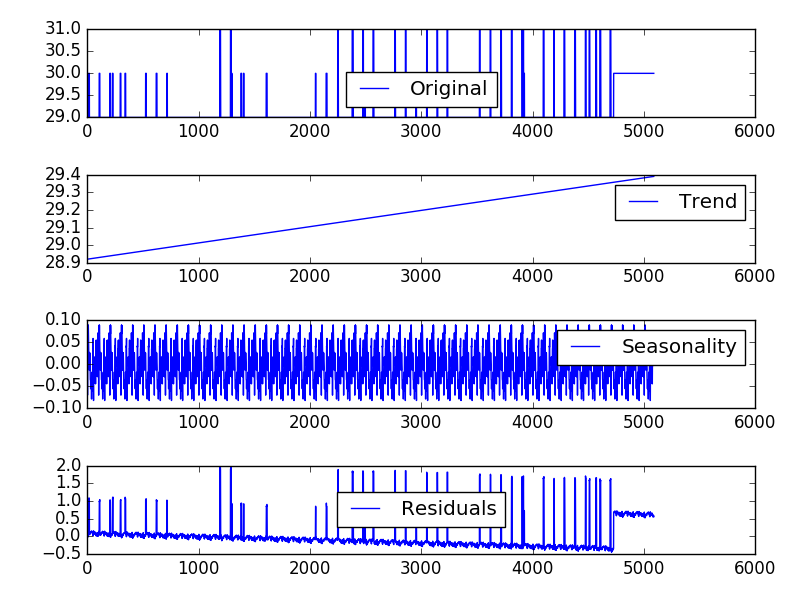
\includegraphics[width=0.9\textwidth]{11506/decomposition.png}
\caption{Decomposition of time series into trend and seasonal component).} \label{fg:decomp}
\end{figure}

\begin{figure}
\subfloat{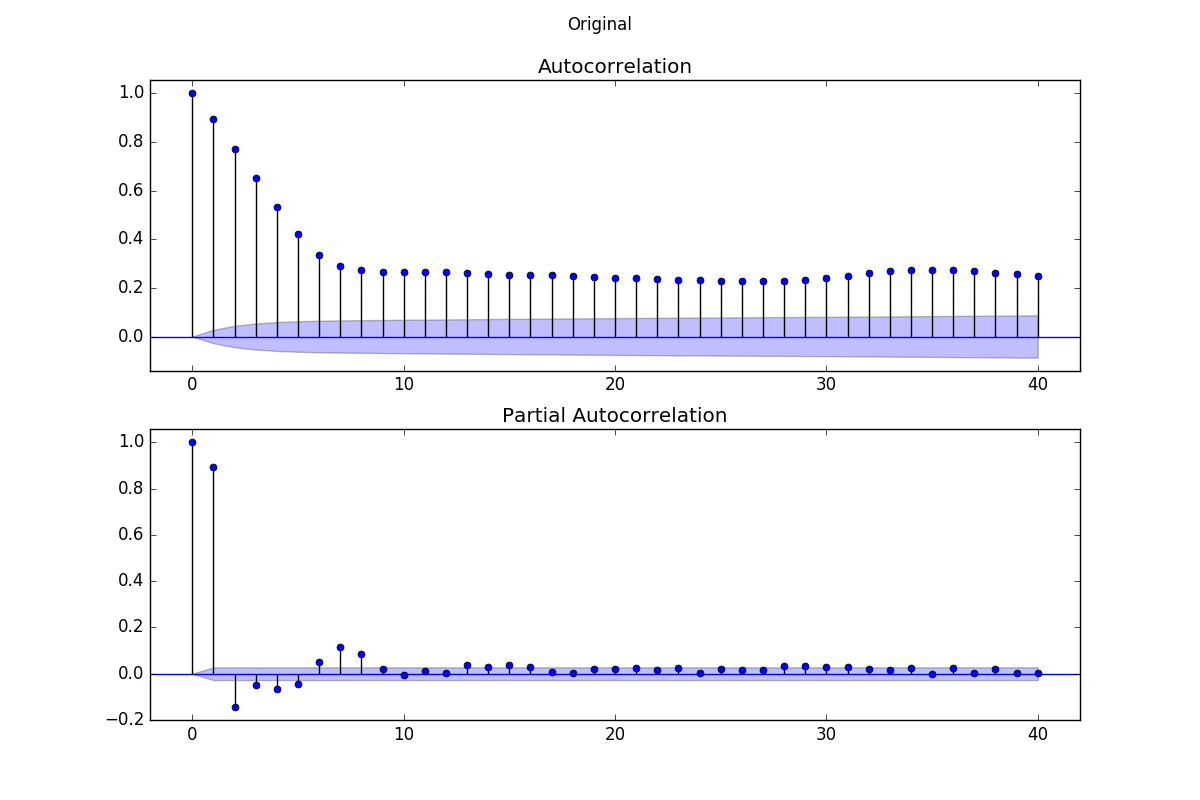
\includegraphics[width=0.5\textwidth]{11506/acf_Original.png}}
\subfloat{\includegraphics[width=0.5\textwidth]{11506/acf_Trend.png}}\\ 
\subfloat{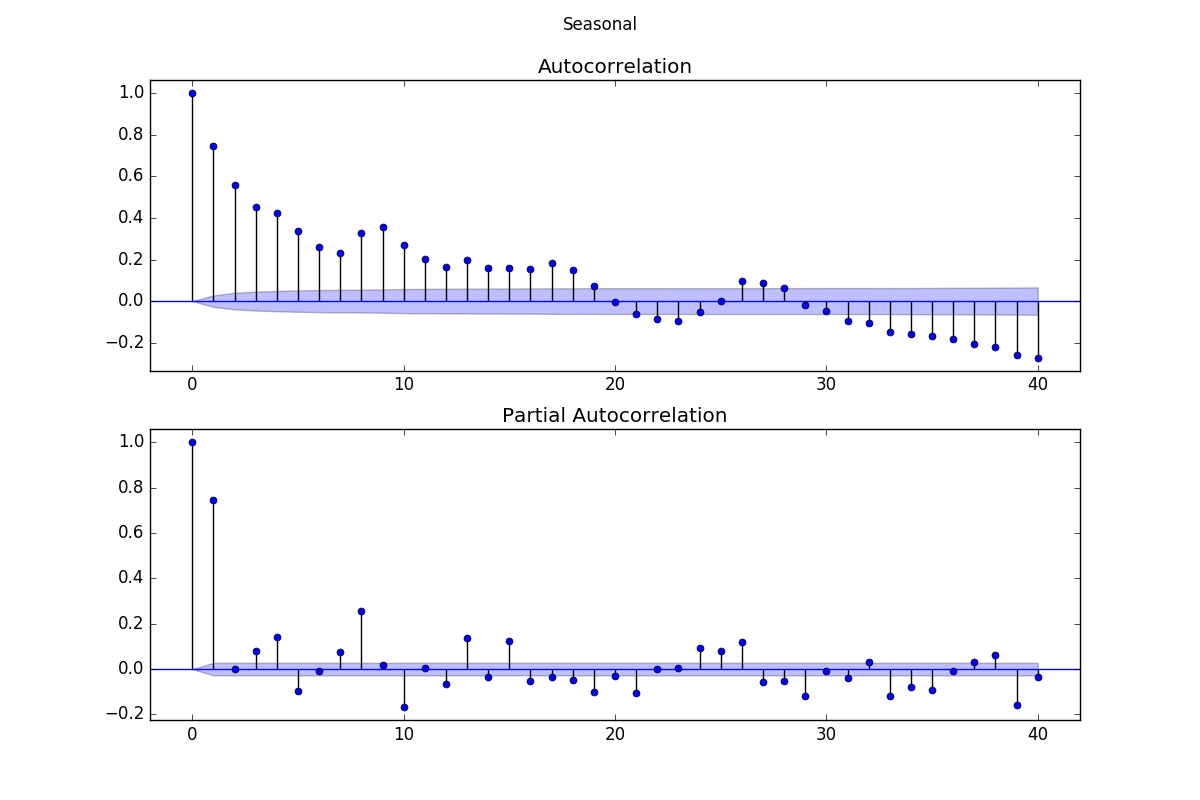
\includegraphics[width=0.5\textwidth]{11506/acf_Seasonal.png}}
\subfloat{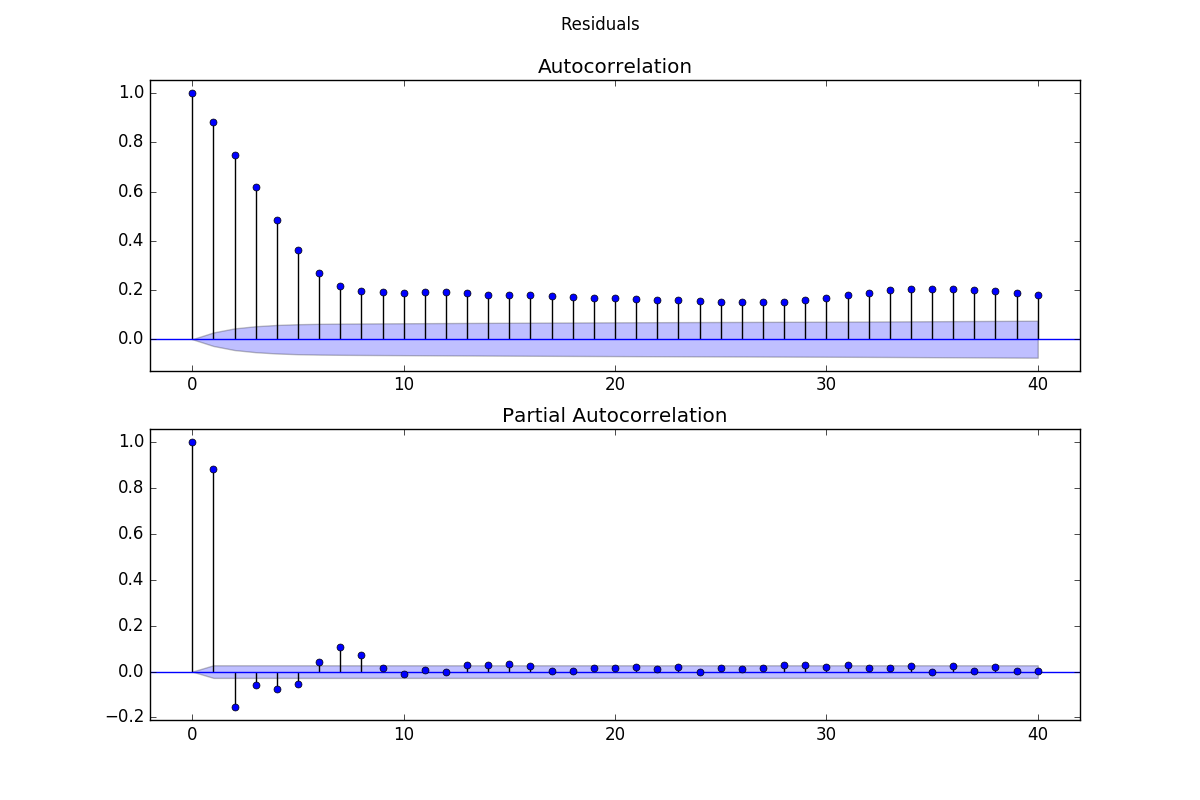
\includegraphics[width=0.5\textwidth]{11506/acf_Residuals.png}}
\caption{ACF and PACF for componets of the time series.} \label{fg:acf}
\end{figure}
11508: Estimated period 100.0 with std 0.0 \\ 

\begin{figure}
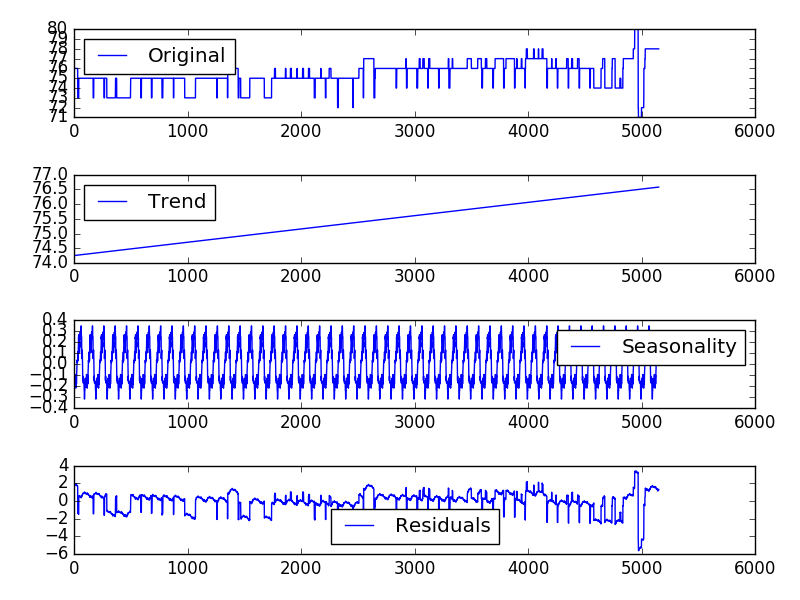
\includegraphics[width=0.9\textwidth]{11508/decomposition.png}
\caption{Decomposition of time series into trend and seasonal component).} \label{fg:decomp}
\end{figure}

\begin{figure}
\subfloat{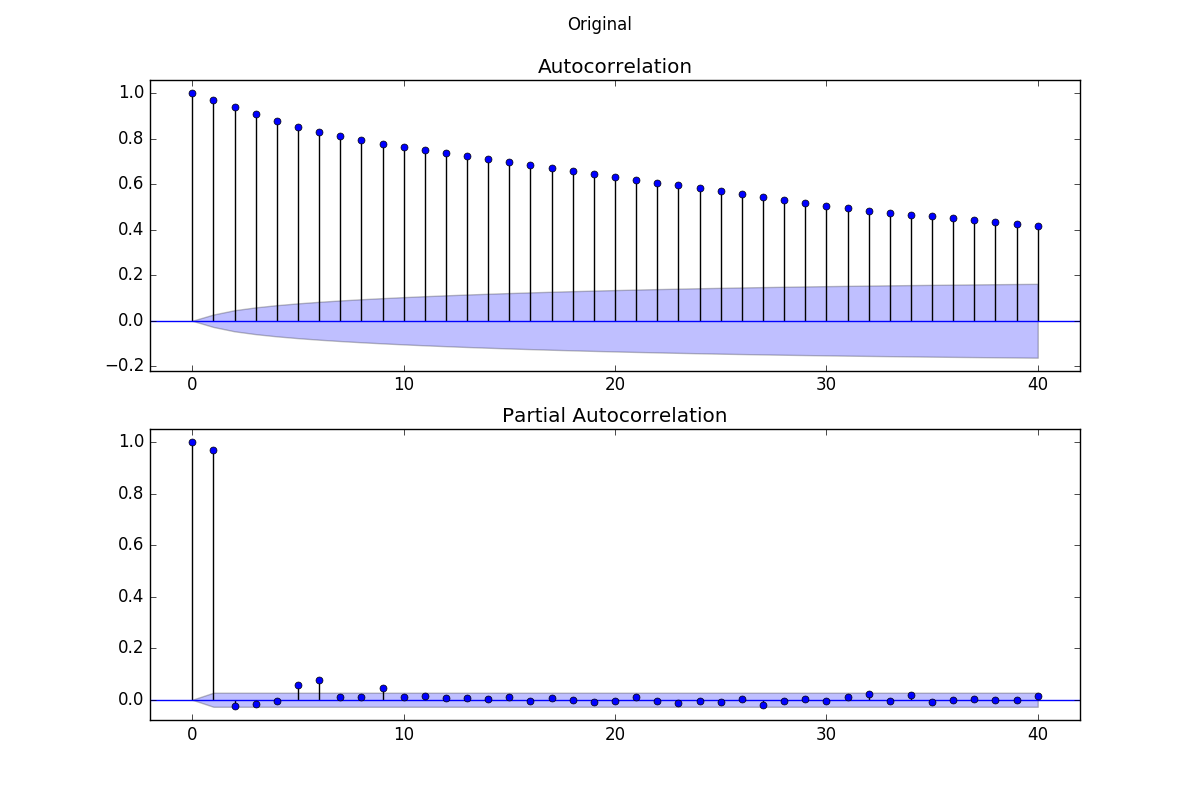
\includegraphics[width=0.5\textwidth]{11508/acf_Original.png}}
\subfloat{\includegraphics[width=0.5\textwidth]{11508/acf_Trend.png}}\\ 
\subfloat{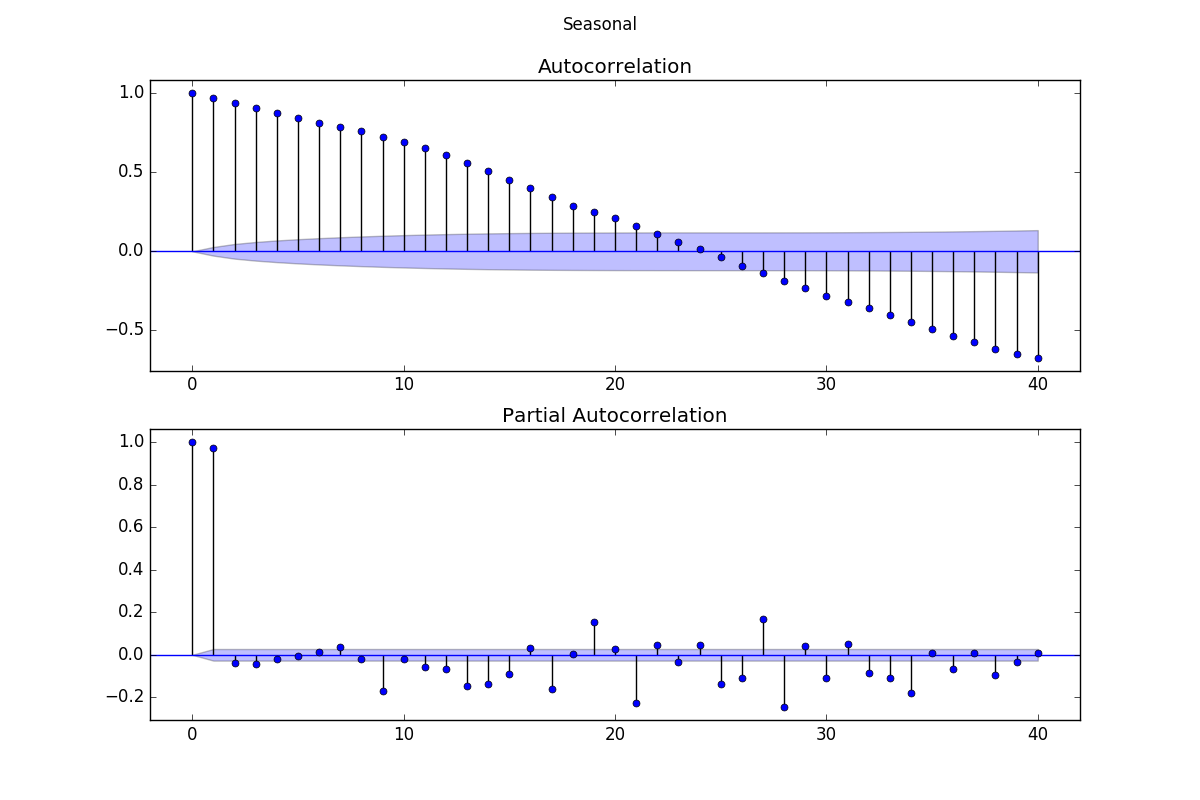
\includegraphics[width=0.5\textwidth]{11508/acf_Seasonal.png}}
\subfloat{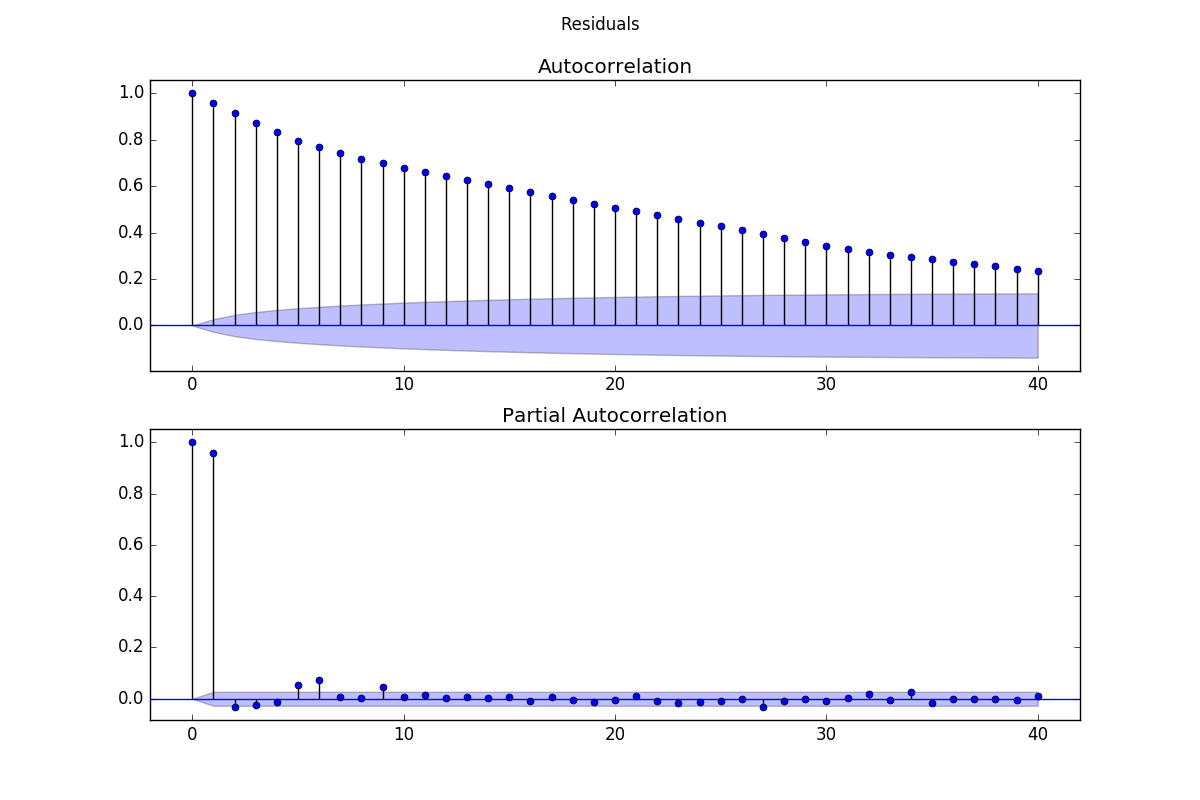
\includegraphics[width=0.5\textwidth]{11508/acf_Residuals.png}}
\caption{ACF and PACF for componets of the time series.} \label{fg:acf}
\end{figure}
11507: Estimated period 100.0 with std 0.0 \\ 

\begin{figure}
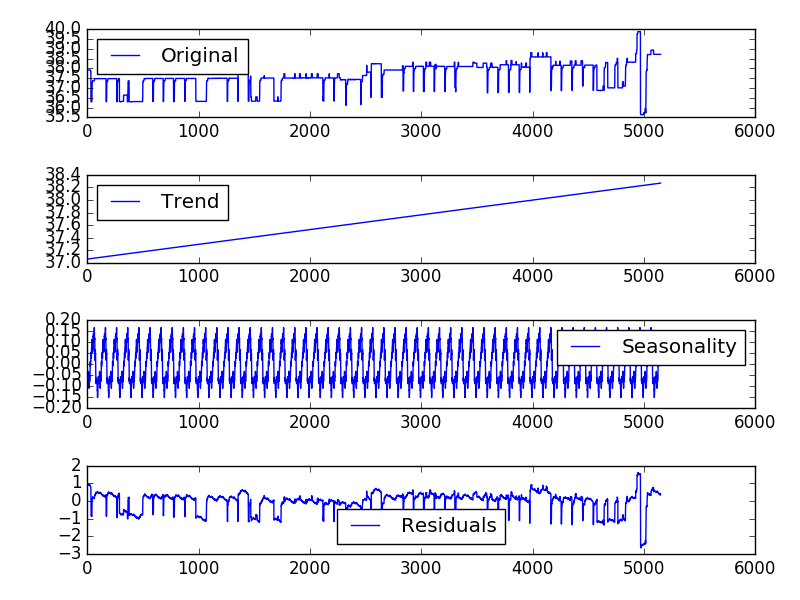
\includegraphics[width=0.9\textwidth]{11507/decomposition.png}
\caption{Decomposition of time series into trend and seasonal component).} \label{fg:decomp}
\end{figure}

\begin{figure}
\subfloat{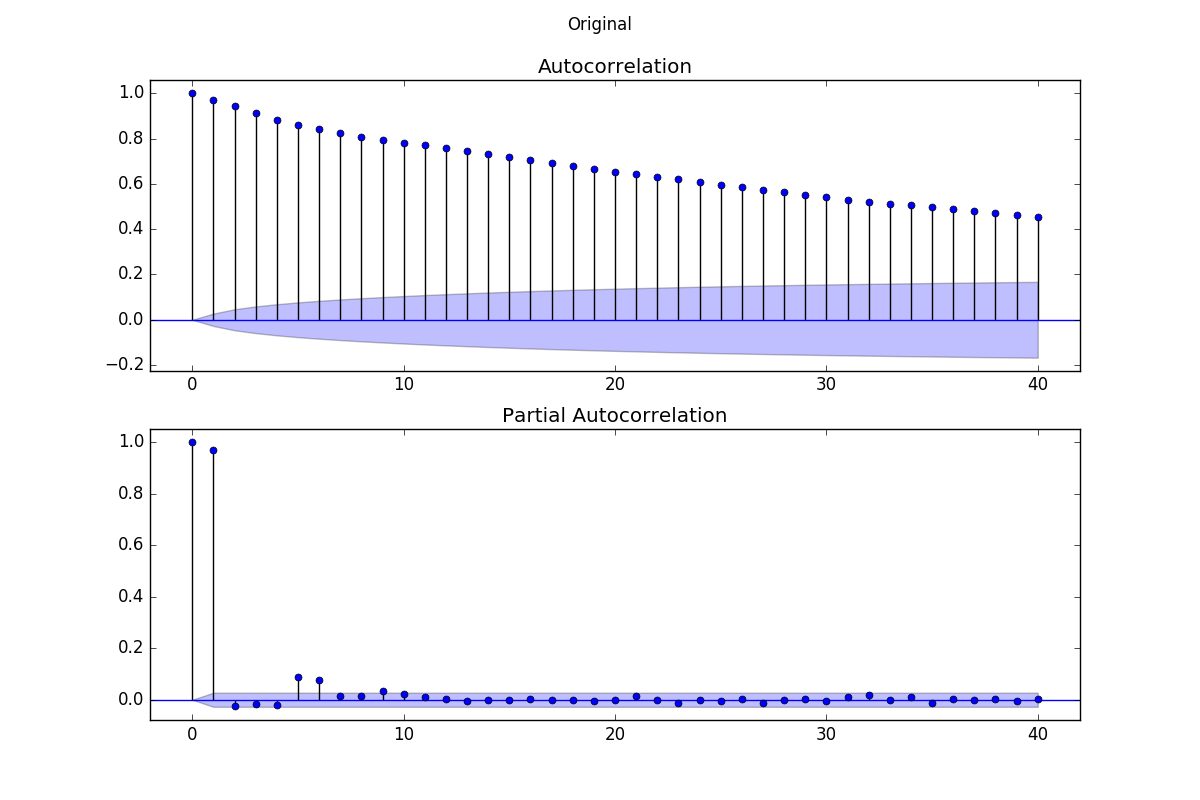
\includegraphics[width=0.5\textwidth]{11507/acf_Original.png}}
\subfloat{\includegraphics[width=0.5\textwidth]{11507/acf_Trend.png}}\\ 
\subfloat{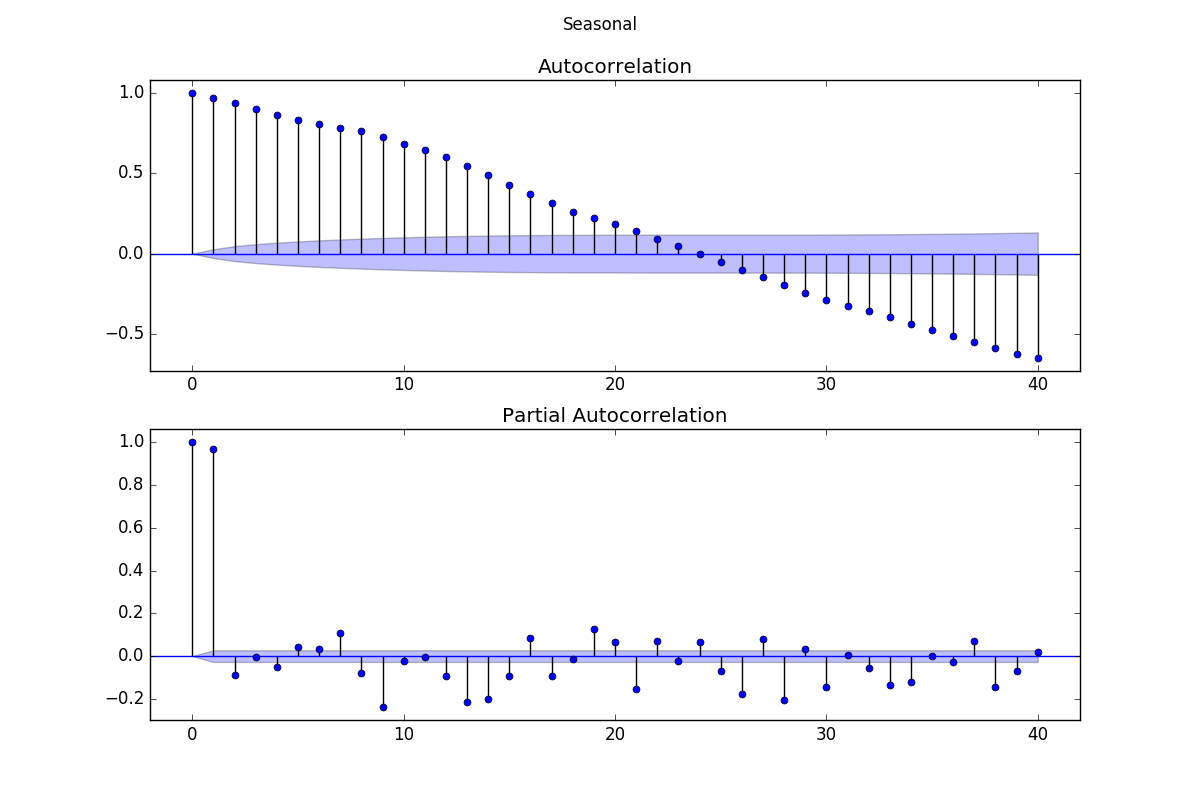
\includegraphics[width=0.5\textwidth]{11507/acf_Seasonal.png}}
\subfloat{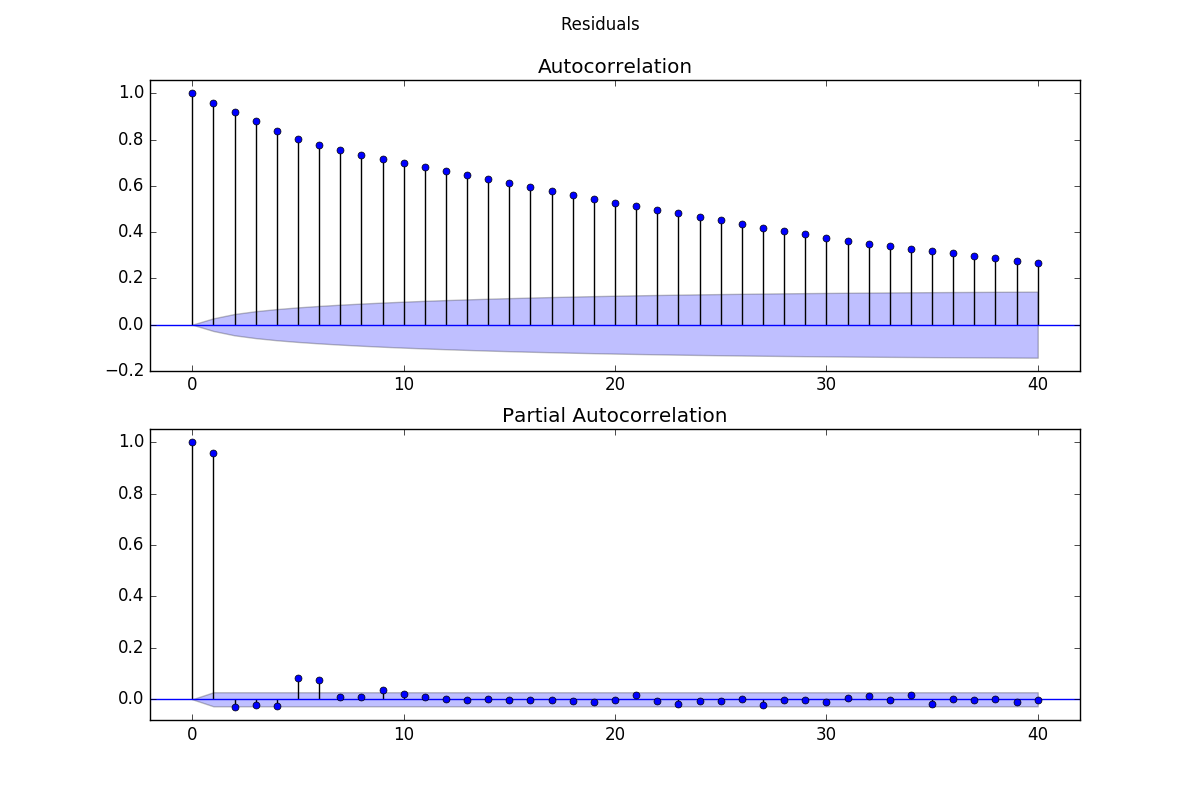
\includegraphics[width=0.5\textwidth]{11507/acf_Residuals.png}}
\caption{ACF and PACF for componets of the time series.} \label{fg:acf}
\end{figure}
Lasso. Best CV error: 0.0143885464155, estimated parameters: history = 2, alpha = 0.0001 \\ 
Lasso\_None\_None\\ 
Train error for estimated parameters: 0.00947418348423, test error with estimated parameters 0.0151400144747 \\ 
\begin{tabular}{lrrrr}
\toprule
{} &  (MAE, train) &  (MAPE, train) &  (MAE, test) &  (MAPE, test) \\
\midrule
11473 &      0.156846 &       0.001085 &     0.225898 &      0.001563 \\
11474 &      0.038419 &       0.001027 &     0.059565 &      0.001591 \\
11505 &      0.228191 &       0.001958 &     0.525350 &      0.004521 \\
11506 &      0.076287 &       0.002564 &     0.198445 &      0.006618 \\
11508 &      0.137154 &       0.001834 &     0.222437 &      0.002938 \\
11507 &      0.068729 &       0.001849 &     0.105797 &      0.002803 \\
\bottomrule
\end{tabular}
\bigskip 
 \\
\begin{figure}
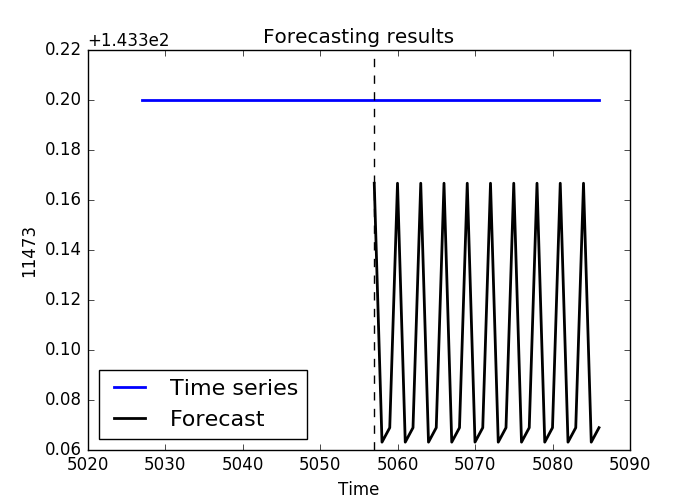
\includegraphics[width=0.7\textwidth]{1477928186/Lasso/11473.png}
\caption{1477928186/Lasso/11473.png.} \label{fg:1477928186/Lasso/11473.png}
\end{figure}

\begin{figure}
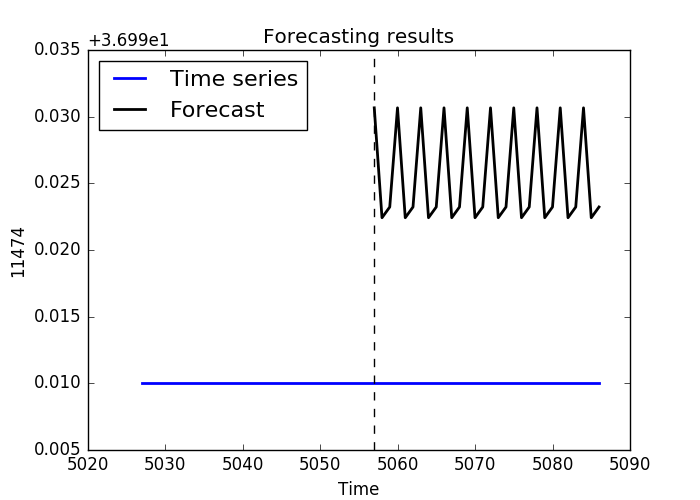
\includegraphics[width=0.7\textwidth]{1477928186/Lasso/11474.png}
\caption{1477928186/Lasso/11474.png.} \label{fg:1477928186/Lasso/11474.png}
\end{figure}

\begin{figure}
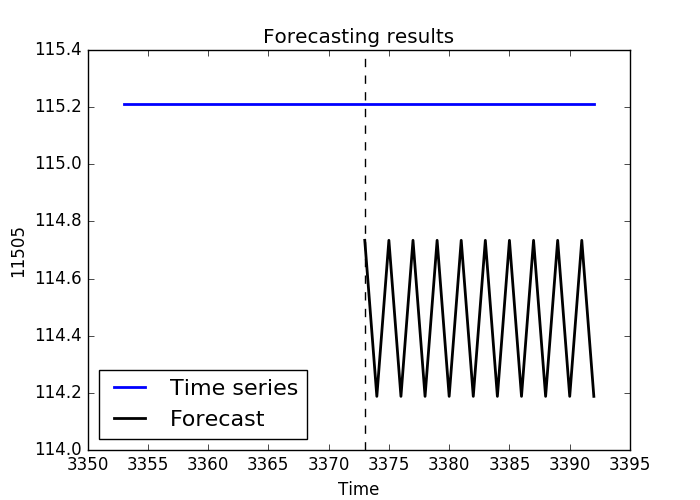
\includegraphics[width=0.7\textwidth]{1477928186/Lasso/11505.png}
\caption{1477928186/Lasso/11505.png.} \label{fg:1477928186/Lasso/11505.png}
\end{figure}

\begin{figure}
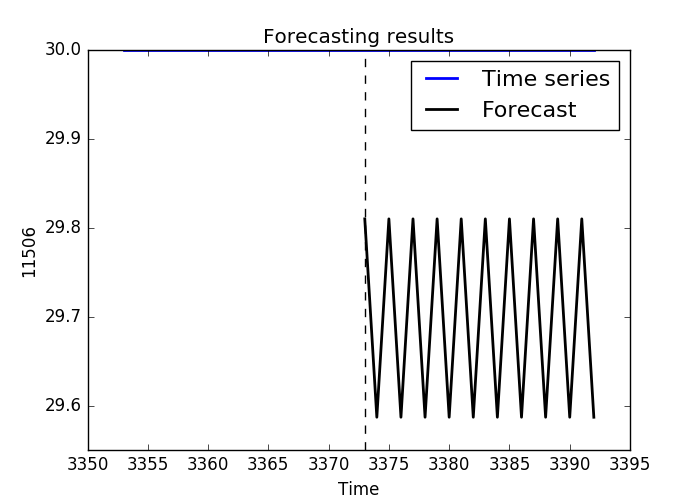
\includegraphics[width=0.7\textwidth]{1477928186/Lasso/11506.png}
\caption{1477928186/Lasso/11506.png.} \label{fg:1477928186/Lasso/11506.png}
\end{figure}

\begin{figure}
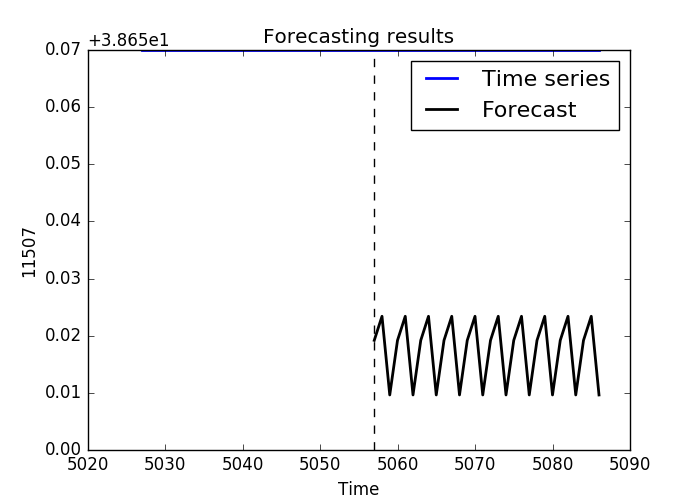
\includegraphics[width=0.7\textwidth]{1477928186/Lasso/11507.png}
\caption{1477928186/Lasso/11507.png.} \label{fg:1477928186/Lasso/11507.png}
\end{figure}

\begin{figure}
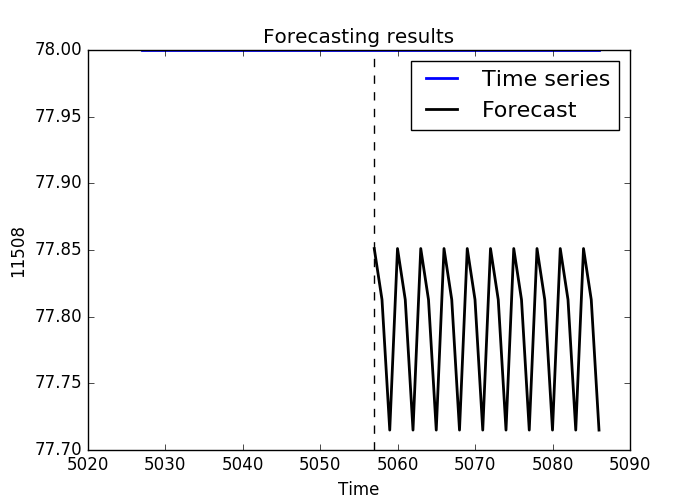
\includegraphics[width=0.7\textwidth]{1477928186/Lasso/11508.png}
\caption{1477928186/Lasso/11508.png.} \label{fg:1477928186/Lasso/11508.png}
\end{figure}

\begin{figure}
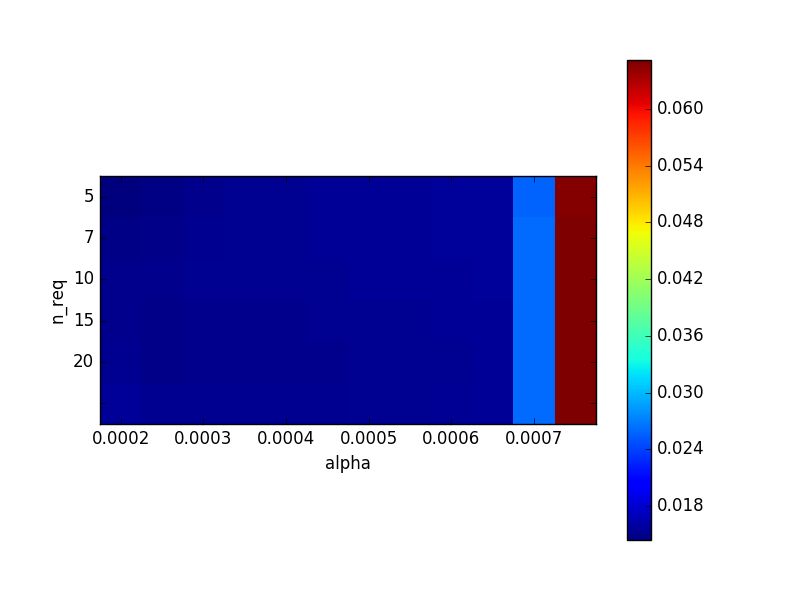
\includegraphics[width=0.7\textwidth]{1477928186/Lasso/cv_optimization.png}
\caption{1477928186/Lasso/cv\_optimization.png.} \label{fg:1477928186/Lasso/cv_optimization.png}
\end{figure}

 Total time: 29.9012789726
 \
\end{document}